\documentclass[ngerman,inputenc]{beamer}

\usepackage{amsmath, amssymb}
\usepackage{appendix}
\usepackage{booktabs}
\usepackage{pstricks}
\usepackage[utf8]{inputenc}
\usepackage{tikz}

\usepackage{graphicx} %package to manage images
\graphicspath{{images/}}

\definecolor{darkblue}{cmyk}{1.0,0.3,0,0.5}
\definecolor{darkred}{cmyk}{0.25,1,0.1,0.1}
\definecolor{uniblau}{cmyk}{1.0,0.7,0.1,0.6}
\definecolor{unihellblau}{cmyk}{0.2,0.14,0,0}
\definecolor{unihellhellblau}{cmyk}{0.05,0.035,0,0}
\definecolor{darkerblue}{cmyk}{1.0,0.3,0,0.7}

\setbeamertemplate{headline}{
\setbeamercolor{author in head/foot}{fg=white,bg=uniblau!80}
 \hbox{%
  \begin{beamercolorbox}[wd=\paperwidth,ht=2.25ex,dp=1ex,left]{author in head/foot}%
    \usebeamerfont{author in head/foot} \hspace{3pt} \insertsection%
  \end{beamercolorbox}
  }
}

\setbeamertemplate{frametitle}
{
    \setbeamercolor{frametitle}{fg=white,bg=uniblau}
    \vspace{-0.1em}
  \begin{beamercolorbox}[wd=\paperwidth,ht=3ex,dp=2ex,left]{frametitle}%
    \usebeamerfont{frametitle}\hspace{0.7em} \textbf{\insertframetitle}%
  \end{beamercolorbox}%
}

\setbeamertemplate{footline}
{
  \leavevmode
   \hspace{-1em}
  \hbox{%
    \setbeamercolor{author in head/foot}{fg=white,bg=uniblau!60}
  \begin{beamercolorbox}[wd=.42\paperwidth,ht=2.25ex,dp=1	ex,center]{author in head/foot}%
    \usebeamerfont{author in head/foot}\insertshortauthor~~(\insertshortinstitute)
  \end{beamercolorbox}%
  \hspace{-1em}
\setbeamercolor{title in head/foot}{fg=white,bg=uniblau!80}
  \begin{beamercolorbox}[wd=.35\paperwidth,ht=2.25ex,dp=1ex,center]{title in head/foot}%
    \usebeamerfont{title in head/foot}\insertshorttitle
  \end{beamercolorbox}%
  \hspace{-1em}
  \setbeamercolor{date in head/foot}{fg=white,bg=uniblau}
  \begin{beamercolorbox}[wd=.25\paperwidth,ht=2.25ex,dp=1ex,right]{date in head/foot}%
    \usebeamerfont{date in head/foot}\insertshortdate{}\hspace*{1em}
    \insertframenumber{} /
    \inserttotalframenumber\hspace*{2ex}
  \end{beamercolorbox}}%
  \vskip0pt%
}

\let\ueberschrift=\frametitle
\renewcommand\frametitle[1]{%
  \ueberschrift{
  \rput[l](0,0){#1}
  }
}

\usecolortheme[named=uniblau]{structure}

\title[Airbnb Oslo]{Price Predictions on Airbnb Accomodations in Oslo, Norway}
\date{21.02.2022}
\author[Freitag, Beck]{Marei Freitag, Joel Beck}
\institute[University Göttingen]{Georg-August-University of Göttingen}

% display TOC before every section and subsection without duplicates
% https://stackoverflow.com/questions/2795478/latex-beamer-prevent-showing-the-toc-at-one-occasion

\RequirePackage{ifthen}
\newboolean{sectiontoc}
\setboolean{sectiontoc}{true} % default to true

\AtBeginSection[]
{
  \ifthenelse{\boolean{sectiontoc}}{
  \begin{frame}
    \frametitle{Table of Contents}
    \tableofcontents[currentsection, currentsubsection, subsubsectionstyle={show/show/shaded/shaded}]
  \end{frame}
  }
}

\AtBeginSubsection[]
{
  \begin{frame}
    \frametitle{Table of Contents}
    \tableofcontents[currentsection, currentsubsection, subsubsectionstyle={show/show/shaded/shaded}]
  \end{frame}
}

\newcommand{\toclesssection}[1]{
  \setboolean{sectiontoc}{false}
  \section{#1}
  \setboolean{sectiontoc}{true}
}


\begin{document}

\begin{frame}
  \titlepage
\end{frame}


\begin{frame}
  \frametitle{Table of Contents}
  \tableofcontents
\end{frame}


\toclesssection{1. Introduction}

\begin{frame}{Introduction}

  Aims of this work:
  \begin{itemize}
    \item Establish a deep learning approach to predict the price of an Airbnb accomodation per night in Oslo, Norway
    \item Focus on explainability and interpretability
  \end{itemize}
  \hspace{12pt}

  $\rightarrow$ Underlying data: provided by Airbnb, contains various information about the listings in Oslo

\end{frame}


\toclesssection{2. Methods}

\subsection{2.1 Preprocessing}

\subsubsection{Feature Engineering}

\begin{frame}{Feature Engineering: Images}

  \begin{itemize}
    \item Use transfer learning on a pretrained CNN (\texttt{ResNet18}) with the first 5 images per listing as input data
    \item Added Fully Connected Network at the end containing three layers and \texttt{ReLU} activation functions to be sure the CNN is able to generalize
    \item Also implemented CNN manually as a benchmark model to compare the results
  \end{itemize}

  \pause

  \hspace{5pt}

  Results:
  \begin{itemize}
    \item pretrained \texttt{ResNet18} achieved a Mean Absolute Error of $579$ NOK (approx. $58$ Euros) on the validation set
    \item But correlation of the CNN predictions with the true price is $0.41$
  \end{itemize}

\end{frame}

\begin{frame}{Image Predictions}

  \begin{figure}[H]
    \centering
    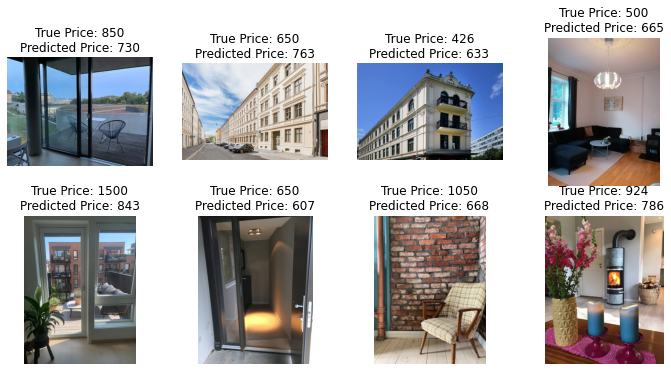
\includegraphics[width=10cm]{cnn_examples_medium.png}
    \caption{CNN example predictions}
  \end{figure}

\end{frame}


\begin{frame}{Feature Engineering: Reviews}
  % Language and Sentiment
  \begin{itemize}
    \item Language: Detect language of each review
    \item Sentiment analysis: Get the sentiment of each review
  \end{itemize}

  \pause

  \hspace{5pt}

  New features per listing:
  \begin{itemize}
    \item[1.] Number of reviews
    \item[2.] Median review length
    \item[3.] Number of different languages of the reviews as well as a list of the different languages
    \item[4.] Fraction of Norwegian and English reviews
    \item[5.] Ratio of negative reviews to the total number of reviews
  \end{itemize}

\end{frame}

\begin{frame}{Wordclouds of the Reviews}

  % Wordcloud
  \begin{figure}[t]
    \centering
    \begin{minipage}{7cm}
      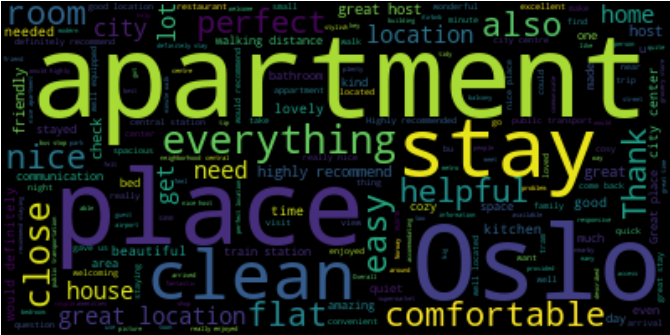
\includegraphics[width=\columnwidth]{wordcloud_eng.png}
    \end{minipage}
    \begin{minipage}{7cm}
      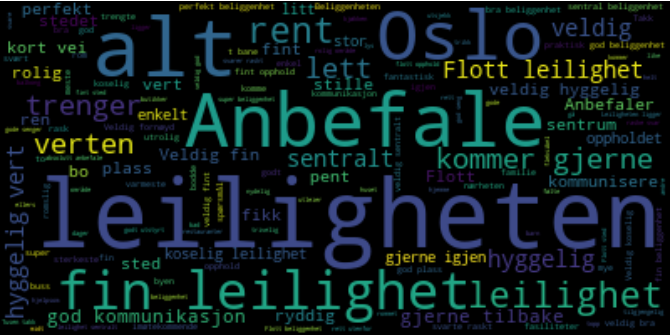
\includegraphics[width=\columnwidth]{wordcloud_nor.png}
    \end{minipage}
  \end{figure}

\end{frame}


\subsubsection{Feature Selection}

\begin{frame}{Feature Selection \& Data Cleaning}

  Feature Selection:
  \begin{itemize}
    \item[1.] Manually selected features based on background knowledge, correlation analysis and the number of missing values
    \item[2.] Adjusted these features by analyzing the results of different feature selection algorithms and fitted auxiliary linear regression
  \end{itemize}

  \pause

  \hspace{5pt}

  Data Cleaning:
  \begin{itemize}
    \item Converting data types
    \item Splitting text-based variables into more convenient numeric or boolean features
    \item Aggregating rare categories of categorical variables into one larger \emph{Other} group to stabilize estimation
    \item One-Hot encoding of categorial variables and standardization of numerical variables
  \end{itemize}

\end{frame}


%%% Models %%%

\subsection{2.2 Models}

\subsubsection{Classical Models}

\begin{frame}{Classical Models}
  \begin{itemize}
    \item[1.] \textbf{Linear Regression}: simple, well understood in terms of underlying theory and highly interpretable.
    \item[2.] \textbf{Ridge Regression}: still very interpretable with a closed form analytical solution
    \item[3.] \textbf{Random Forest}: very flexible model, can be applied to many contexts and often works 'out of the box'
    \item[4.] \textbf{Histogram-Based Gradient Boosting}: modern and fast tree-based gradient boosting algorithm; similar to Random Forest, but uses Boosting instead of Bagging
  \end{itemize}

\end{frame}


\subsubsection{Neural Network}

\begin{frame}{Neural Network: Model Architecture}

  \begin{columns}
    \begin{column}{0.5\textwidth}
      \begin{itemize}
        \item Linear input layer (about $60$ features)
        \item $6$ intermediary \textbf{blocks} with $64$, $128$, $256$, $128$, $64$ and $8$ output features:
              \begin{itemize}
                \item[–] Residual connection
                \item[–] Linear layer with BatchNorm, \texttt{ReLU} activation function and dropout
              \end{itemize}
        \item $1$ output neuron
      \end{itemize}
    \end{column}
    \begin{column}{0.5\textwidth}
      \begin{center}
        \begin{figure}
          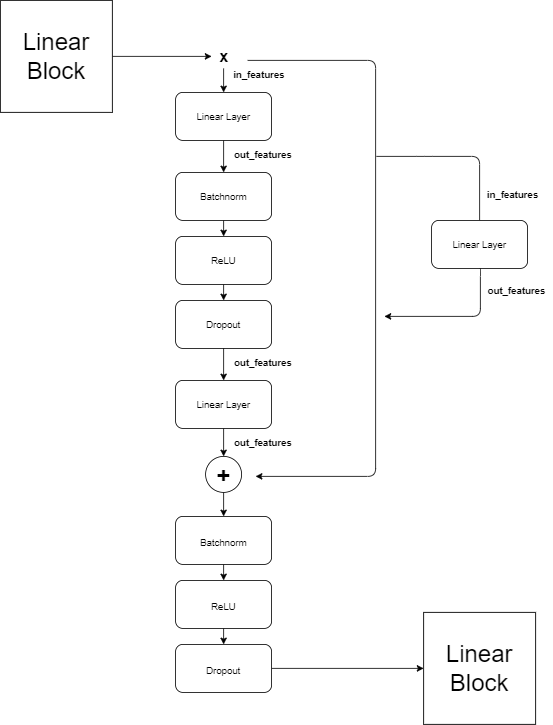
\includegraphics[width=0.95\columnwidth]{mlp_architecture.png}
        \end{figure}
      \end{center}
    \end{column}
  \end{columns}

\end{frame}

\begin{frame}{Neural Network: Model Training}

  \begin{itemize}
    \item Optimizer: \texttt{Adam} with learning rate set to 0.01
    \item Loss function: \textit{Mean Squared Error} Loss
    \item Epochs: Number of epochs vary; stopped training if Loss stagnated or model began to overfit
  \end{itemize}

  \pause

  \hspace{5pt}

  Most impactful hyperparameter: \textbf{Dropout rate}

  \begin{itemize}
    \item[–] high influence of the network's generalizatioin availability
    \item[–] model overfitted significantly by setting dropout rate to zero \\
      $\rightarrow$ that shows the current model structure is flexible enough to model the task properly
    \item[–] increasing the rate leads to higher training MAE but also improves the model's performance on the validation set
  \end{itemize}


\end{frame}



\toclesssection{3. Results}

\subsection{3.1 Evaluation Metrics}

\begin{frame}{Evaluation Metrics}
  \begin{itemize}
    \item Focus on Mean Absolute Error and $R^2$ for higher \textbf{interpretability} \pause
    \item Computations of MAE and $R^2$ on \textbf{original} price scale  \\
          $\Rightarrow$ requires backtransformation of fitted values when using \textbf{log-price}\pause
    \item Values depend on exact evaluation procedure, direct comparisons across groups have to be taken with care
          \begin{align*}
            MAE \left(\mathbf{y}, \exp \left(\widehat{\log(\mathbf{y})}\right)\right)
             & \neq \exp \left(MAE \left(\log(\mathbf{y}), \widehat{\log(\mathbf{y})}\right) \right) \\
            R^2 \left(\mathbf{y}, \exp \left(\widehat{\log(\mathbf{y})}\right)\right)
             & \neq R^2 \left(\log(\mathbf{y}), \widehat{\log(\mathbf{y})}\right)
          \end{align*}
  \end{itemize}
\end{frame}

\subsection{3.2 Predictive Performance}

\begin{frame}{Training \& Validation Performance}
  \begin{figure}[h]
    \centering
    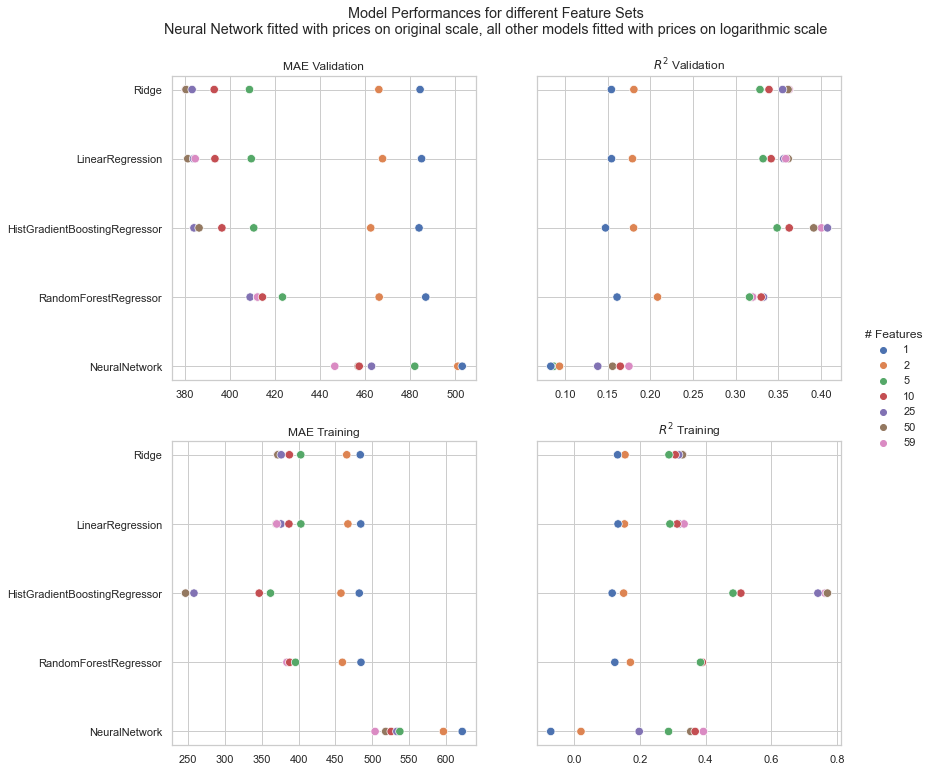
\includegraphics[width=0.8\textwidth]{model_comparison.png}
    \label{fig:model-comparison}
  \end{figure}
\end{frame}

\begin{frame}{Main Findings}
  \begin{itemize}
    \item More features tend to work better with diminishing returns ($5$ vs. all features)
    \item Price prediction task with small tabular data does not require overly complex models \\
          $\Rightarrow$ similar performance of linear and nonlinear classical models,  linear models generalize better to validation set
    \item Neural Net: At first sight worst performance but best generalization \\
          $\Rightarrow$ Differing behaviour of \emph{Dropout} and \emph{Batchnorm} layers during training and inference $+$ presence of outliers
  \end{itemize}
\end{frame}

\begin{frame}{Main Findings}
  \begin{itemize}
    \item Without outlier removal we can expect a MAE of $400$ NOK (40 Euros) and a $R^2$ value of around $0.4$.
    \item Validation performance is biased towards models whose hyperparameters were tuned during cross validation
  \end{itemize}
\end{frame}

\begin{frame}{Test Set Performance}
  \begin{table}[h]
    \centering
    \begin{tabular}{lrr}
      \hline
      Model                & \multicolumn{1}{c}{MAE} & \multicolumn{1}{c}{$R^2$} \\ \hline
      Linear Regression    & 404.709                 & 0.298                     \\
      Ridge                & 405.932                 & 0.294                     \\
      Random Forest        & 444.166                 & 0.268                     \\
      HistGradientBoosting & 412.243                 & 0.387                     \\
      Neural Network       & 402.24                  & 0.333                     \\
      Top2 Average         & 404.848                 & 0.296                     \\
      Top3 Average         & 399.315                 & 0.343                     \\
      Top4 Average         & 404.206                 & 0.332                     \\
      Top5 Average         & 408.116                 & 0.27                      \\ \hline
    \end{tabular}
    \caption{Test Set Performance of Classical Machine Learning Models, our custom Neural Network and Ensemble Predictions}
    \label{tab:test-set}
  \end{table}
\end{frame}

\subsection{3.3 Understanding \& Interpretation}

\subsubsection{Feature Importance}

\begin{frame}{Feature Importance}
  \begin{columns}
    \begin{column}{0.6\textwidth}
      \begin{center}
        \begin{figure}
          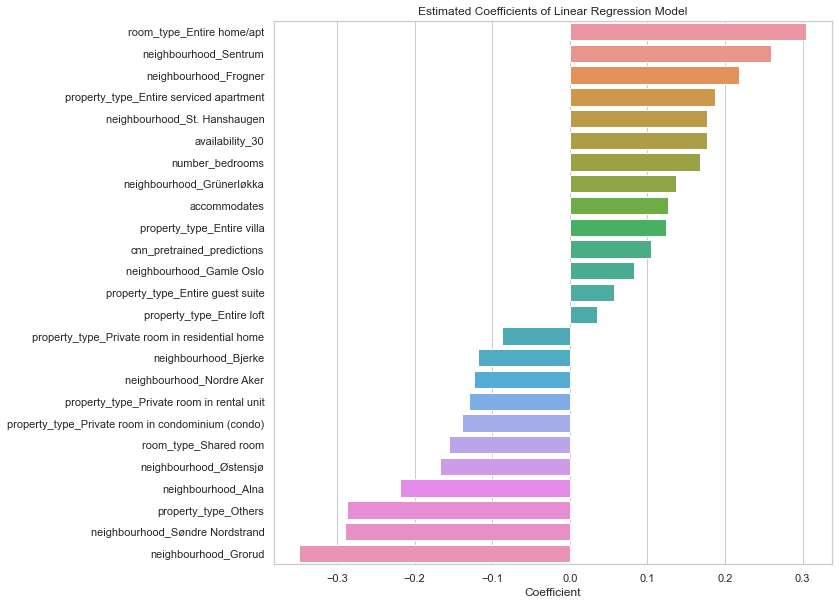
\includegraphics[width=\columnwidth, height=0.75\textheight]{coefficient_plot.png}
          \label{fig:coefficient-plot}
        \end{figure}
      \end{center}
    \end{column}
    \begin{column}{0.4\textwidth}
      \begin{itemize}
        \item Largest (absolute) Coefficients: \emph{room type}, \emph{property type} and \emph{neighbourhood}
        \item Top $2$ by Feature Selector: \emph{number of bedrooms} and \emph{accomodates}
        \item Marginal vs. Conditional Impact (\emph{Sentrum} neighbourhood)
      \end{itemize}
    \end{column}
  \end{columns}
\end{frame}


\subsubsection{Sensitivity to Outliers}

\begin{frame}{Impact of Outliers}
  \begin{table}[t]
    \centering
    \begin{tabular}{@{}ccc@{}}
      \toprule
      Quantile Threshold & MAE    & $R^2$ \\ \midrule
      0.0                & 443.35 & 0.16  \\
      1.0                & 337.59 & 0.51  \\
      2.5                & 282.17 & 0.53  \\
      5.0                & 240.57 & 0.54  \\
      10.0               & 214.76 & 0.49  \\ \bottomrule
    \end{tabular}
    \caption{MAE and $R^2$ value of the Neural Network on the validation set}
    \label{tab:mlp-outliers}
  \end{table}
  \pause
  \begin{itemize}
    \item \textbf{Not} fixed by log-transformation!
    \item Explains performance boost of Neural Network from training to validation to test set
  \end{itemize}
\end{frame}

\begin{frame}{Impact of Outliers}
  \begin{itemize}
    \item In theory the Neural Net should be flexible enough to approximate any arbitrary function reasonably well
    \item Why is it not able to capture entire price range? \pause
    \item Model only uses features during prediction \\
          $\Rightarrow$ To \textbf{discriminate} between outliers and non-outliers, the corresponding feature combinations must be \textbf{separable} in high-dimensional feature space
    \item Idea: approximate full feature space by two-dimensional \textbf{embedding}
  \end{itemize}
\end{frame}

\begin{frame}{Feature Space Embedding}
  \begin{figure}[t]
    \centering
    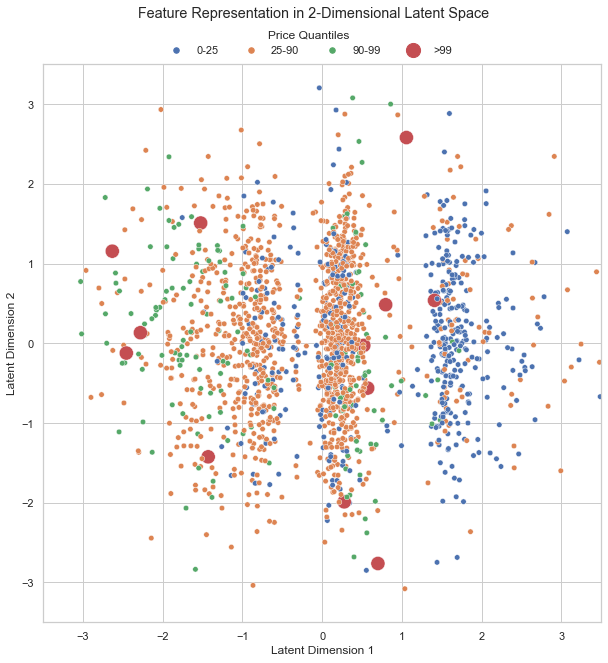
\includegraphics[width=0.6\textwidth]{latent_representation.png}
    \label{fig:latent-representation}
  \end{figure}
\end{frame}

\begin{frame}{Takeaways}
  \begin{itemize}
    \item Why is there no separability?
          \begin{enumerate}
            \item Data is not rich/expressive enough to capture all factors that contribute to very high prices
            \item Some apartments are listed at a price that does not represent their \textbf{true} value
          \end{enumerate}
          \pause
    \item Can't we just remove those outliers?
          \begin{itemize}
            \item Expensive, but \textbf{fairly priced} observations should be kept \\
                  $\Rightarrow$ Might be contained in prediction tasks on new data, thus model should learn to handle those cases during training
            \item Detecting (and removing) truly \textbf{overpriced} observations is difficult (many reasons for e.g. low demand)
          \end{itemize}
  \end{itemize}
\end{frame}


\section{4. Munich Data}

\begin{frame}{Munich - Predictive Performance}
  \begin{itemize}
    \item About twice as large as Oslo Data \\
          $\Rightarrow$ Flexible Models like Gradient Boosting and the Neural Network
          benefit most \pause
    \item However: Overall Performance \emph{not} significantly better than for Oslo Data
    \item MAE of Neural Net on validation set from $44.3$ Euros for Oslo to $42.5$ Euros for Munich
    \item Gradient Boosting model with best test set performance: MAE of $32.8$ (Oslo: $41.2$) and $R^2$ of $0.453$ \pause
    \item Deeper/Wider architecture of neural net that is specifically designed for larger data set might lead to performance boost
  \end{itemize}
\end{frame}

\begin{frame}{Munich - Understanding \& Interpretation}
  \begin{itemize}
    \item Most important features: \emph{Property Type}, \emph{Neighbourhood} and \emph{Accomodates} \pause
    \item Munich Data again contains large price outliers with high impact on the evaluation metrics
          \vspace{1em}
          \begin{table}[h]
            \centering
            \begin{tabular}{@{}ccc@{}}
              \toprule
              Quantile Threshold & MAE   & R2   \\ \midrule
              0.0                & 42.49 & 0.31 \\
              1.0                & 35.32 & 0.44 \\
              2.5                & 30.26 & 0.42 \\
              5.0                & 25.2  & 0.45 \\
              10.0               & 22.94 & 0.4  \\ \bottomrule
            \end{tabular}
            \label{tab:munich-outliers}
          \end{table}
  \end{itemize}
\end{frame}


\section{5. Conclusion}

\begin{frame}{Conclusion}
  \begin{itemize}
    \item Linear Models show competitive predictive performance for small Oslo data
    \item Top 3 Ensemble leads to lowest test set error
    \item Large impact of outliers
    \item Extension to gain further understanding of the network's behaviour: \emph{Adversarial Examples} in regression context  \\
          $\Rightarrow$ Find small input \textbf{perturbations} which lead to spike in price predictions
  \end{itemize}
\end{frame}

\begin{frame}{References}
  \tiny
  \nocite{he2015, ioffe2015,kingma2014,kingma2017,srivastava2014,goodfellow2015}
  \bibliographystyle{apalike}
  \bibliography{bib.bib}
\end{frame}

\begin{frame}

  \begin{center}
    \LARGE{\textbf{Thanks for listening!}}\\[10mm]
    \large{Questions?}
  \end{center}

\end{frame}



\end{document}
%